\section{Methodology}

The methodology consists of two connected stages. The first stage replicates the original Java-based SIDE study to examine whether the reported association between SIDE and human judgments can be recovered from the released artifact. The second stage adapts SIDE to Python and uses the resulting metric as a filtering signal for code-summary training data.

\begin{figure*}[t]
    \centering
    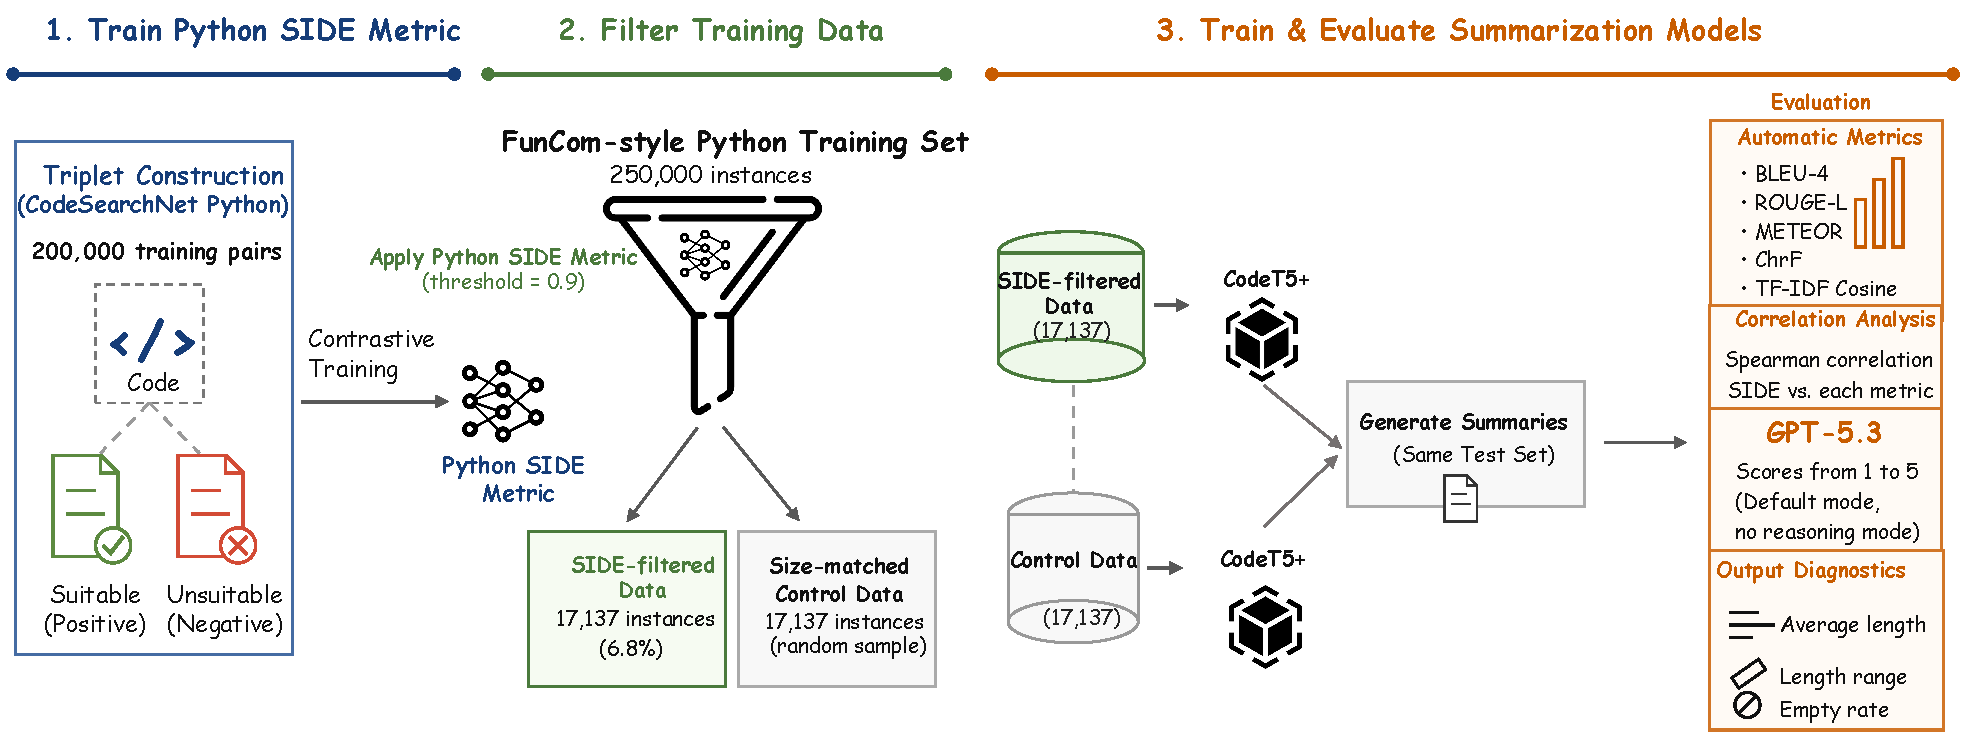
\includegraphics[width=\textwidth]{workflow.pdf}
    \caption{Overview of the Python SIDE extension workflow.}
    \label{fig:python-side-workflow}
\end{figure*}

\subsection{Replication Methodology}

The replication follows the design of the original SIDE paper~\cite{mastropaolo2024evaluating}. The original study frames code summarization evaluation as a code--text alignment problem rather than only as reference-summary matching. In its contrastive formulation, the code fragment serves as the anchor, a suitable summary serves as the positive example, and an unsuitable summary serves as the negative example.

The replication began with artifact recovery. Although the released artifact included the main training, scoring, and statistical-analysis scripts, it was not directly executable in a clean local environment. Some required resources were distributed outside the artifact, and several scripts assumed machine-specific paths or environment variables. The execution environment was therefore reconstructed, the missing training and evaluation resources were restored, and the analysis was rerun locally before comparing the reproduced results with the reported ones.

The SIDE training objective was kept unchanged. The model learns a shared embedding space in which code fragments are closer to suitable summaries than to unsuitable ones. Following the original setup, MPNet is used as the encoder and triplet loss as the contrastive objective. Negative summaries are constructed in two forms: randomly sampled summaries from other examples and hard negatives that remain related to the code but omit part of its behavior. This distinction is important because an incorrect generated summary is often not arbitrary; it may describe the code only partially.

The replication uses the same human-judgment benchmark as the original analysis. The benchmark contains developer ratings for automatically generated summaries of Java methods. Developer-written reference summaries are excluded from the regression analysis, since the comparison is intended to evaluate generated summaries rather than references themselves. After this filtering step, the analysis set contains 5,201 annotated code-summary evaluations.

SIDE is evaluated together with the automatic metrics used in the original study, including lexical-overlap, character-level, embedding-based, and code-summary alignment metrics. This comparison examines whether SIDE behaves similarly to reference-based metrics or captures a distinct aspect of summary quality. The original metric-comparison procedure and statistical modeling pipeline are rerun so that the reproduced results can be compared with the reported findings.

The statistical analysis follows two steps. Relationships among automatic metrics are first examined using rank-based correlation and dimensionality reduction, which indicates whether SIDE clusters with reference-based metrics or forms a separate evaluation dimension. Ordered logistic regression is then used to estimate the association between each metric and the human-rated quality dimensions: direct assessment, content adequacy, conciseness, and fluency. The replicated quantities of interest are odds ratios; values above one indicate that higher metric scores are associated with higher odds of receiving a better human rating.

\subsection{Extension Methodology}

Figure~\ref{fig:python-side-workflow} summarizes the Python extension. In this stage, SIDE is adapted from Java to Python and used as a data-centric filtering signal rather than only as an evaluation metric. The workflow consists of training a Python-specific SIDE metric, filtering Python code-summary pairs, and comparing summarization models trained with and without this filtering step.

Python SIDE is trained with contrastive triplets. Each triplet contains a Python code fragment, its matched ground-truth summary, and a randomly sampled mismatched summary. The code fragment is treated as the anchor, the matched summary as the positive example, and the mismatched summary as the negative example. Training encourages aligned code-summary pairs to have higher cosine similarity than mismatched pairs in the shared semantic space.

After training, the Python SIDE model scores the FunCom-style Python training pairs. A threshold of 0.9 is used to retain only pairs whose code and summary are strongly aligned. Because this filtering changes the size of the training set, a size-matched control set is constructed by randomly sampling the same number of examples from the unfiltered data. This yields two training conditions: a SIDE-filtered set and an unfiltered size-matched control set.

Next, the same CodeT5+ summarization model is trained under both conditions. The architecture and training configuration are fixed across runs, so the comparison isolates the effect of training-data filtering rather than model capacity or optimization choices. Both trained models then generate summaries for the same Python benchmark examples.

The generated summaries are evaluated with BLEU-4, ROUGE-L, METEOR, ChrF, TF-IDF cosine similarity, and SIDE. Spearman correlations are computed between SIDE and the remaining metrics to examine whether SIDE filtering changes the monotonic relationship between semantic alignment and existing evaluation signals. As an additional evaluation signal, GPT-5.3 is used in its default mode, without reasoning mode, as an LLM judge that assigns 1--5 quality scores.

Output-level diagnostics are also computed for both conditions, including average generated-summary length, length range, and empty-summary rate. These measurements help distinguish genuine quality differences from degenerate changes in generation behavior, such as producing shorter or empty summaries.